\newpage
\section{Tilstandslogikk}
\thispagestyle{fancy}

Styring og logikk som skulle skje i kvar tilstand valgte vi å samle i ei funksjonsblokk som vi kaller tilstandslogikk og som fikk navn etter tilstanden
den skulle styre. Desse funksjonsblokkene er skrevet og løyst spesefikt for deira arbeidsoppgåver i programet og kvar
tilstand har eigen funksjonsblokk med tilstandslogikk. \newline
Kvar tilstandslogikk får inn XE (external enable) ifrå tilstandsmaskina som startar tilstandslogikken. Når sekvensen er ferdig sender
funksjonsblokka høg på utgang Y som returerast til tilstandsmaskina som avanserer til neste tilstand og tilstandslogikk.

Det er tilstandslogikken som har ansvar for å samarbeide med IEC-blokkene som vidare
leser inngangssignal, startar og stoppar elektrisk utstyr, kontrollerer feedback, feilmeldingar og skriv akutelle parameter.

\begin{figure}[htbp]
    \centering
    \begin{subfigure}[b]{0.3\textwidth}
        \centering
        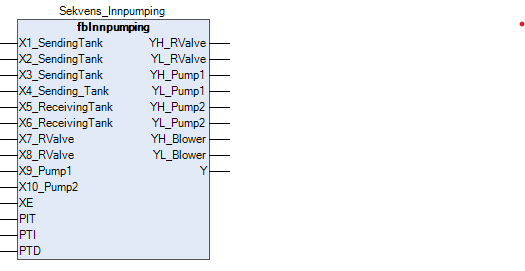
\includegraphics[width=1\textwidth]{Bilder/fbInnpumping.png}
        \caption{Innpumping}\label{fig:fbInnpumping}
    \end{subfigure}
    \hfill
    \begin{subfigure}[b]{0.3\textwidth}
        \centering
        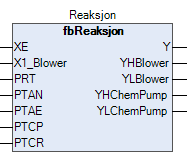
\includegraphics[width=1\textwidth]{Bilder/fbReaksjon.png}
        \caption{Reaksjon}\label{fig:fbReaksjon}
    \end{subfigure}
    \caption{Utklipp av tilstandslogikk}\label{fig:ReaksjonsFasen}
\end{figure}



